\documentclass[]{article}

\author{Braden Fineberg}
\usepackage[pdftex]{graphicx}
\usepackage{achicago}
\usepackage{fullpage}
\usepackage{ amssymb }
\usepackage{amsmath} 
%\usepackage[top=1in, bottom=1in, left= 1 in, right=1in]{geometry}
\usepackage{setspace}
\usepackage[nopar]{lipsum} % for dummy text
\newcommand{\HRule}{\rule{\linewidth}{0.25mm}}

\usepackage{listings}
\usepackage{subfig}
\usepackage{color} %red, green, blue, yellow, cyan, magenta, black, white
\definecolor{mygreen}{RGB}{28,172,0} % color values Red, Green, Blue
\definecolor{mylilas}{RGB}{170,55,241}
\renewcommand\thesection{\Alph{section}}


\begin{document}
	
	\lstset{language=Matlab,%
		%basicstyle=\color{red},
		breaklines=true,%
		morekeywords={matlab2tikz},
		keywordstyle=\color{blue},%
		morekeywords=[2]{1}, keywordstyle=[2]{\color{black}},
		identifierstyle=\color{black},%
		stringstyle=\color{mylilas},
		commentstyle=\color{mygreen},%
		showstringspaces=false,%without this there will be a symbol in the places where there is a space
		numbers=left,%
		numberstyle={\tiny \color{black}},% size of the numbers
		numbersep=9pt, % this defines how far the numbers are from the text
		emph=[1]{for,end,break},emphstyle=[1]\color{red}, %some words to emphasise
		%emph=[2]{word1,word2}, emphstyle=[2]{style},  
		basicstyle=\tiny,  
	}

\input{../title.tex} 

\section{CTMC states}
Given the integer nature of the problem, $X(t)$ will be integer values between 0 and max.

\section{Transition times out of given state}
The transition time will be the first occurrence of anything that changes the value of X. Given that the chance of a claim, premium or dividend is paid are all exponentially distributed, the transition time will also be exponential. Lack of transition is the case in which no event happens. Exponential distributions are additive, therefore, $$T_{leave} = min\{T_p, T_c, T_d\} \qquad T_{stay} = e^{-(\lambda + \alpha + \beta)t}$$
\begin{center}
	\begin{tabular}{|| c | c | c||} 
		\hline
		Range & Event & $v_x$ \\ [0.5ex] 
		\hline\hline
		A & premium & $\lambda$ \\ 
		\hline
		B & premium \& claim paid @ $X(t)$& $\lambda + \alpha$ \\
		\hline
		C & premium \& claim paid & $\lambda + \alpha$ \\
		\hline
		E & claim, dividend & $\lambda + \beta$ \\ [.5ex] 
		\hline
	\end{tabular}
\end{center}

\section{Possible states going out of X(t) = x}
Given that there are only four options for each transition out of x, 
\begin{center}
	\begin{tabular}{|| c | c | c||} 
		\hline
		Range & Event & Possible States \\ [0.5ex] 
		\hline\hline
		A & premium & x+1 \\ 
		\hline
		B & premium \& claim paid @ $X(t)$& x+1, net 0 \\
		\hline
		C & premium \& claim paid & x+1-c \\
		\hline
		E & claim, dividend & x-c-d\\ [.5ex] 
		\hline
	\end{tabular}
\end{center}

\section{Transition probabilities}
Given Baye's theory, 
\begin{center}
	P\{premium payment$|$ a transition happens\} =$\frac{\text{	P\{premium payment\}}\ \cap \text{ P\{transition happens\}}}{\text{P\{transition happens\}}}$
\end{center}
$$= \frac{\lambda}{\lambda+\alpha+\beta }$$
\begin{center}
	\begin{tabular}{|| c | c | c||} 
		\hline
		Range & State j & Transition P \\ [0.5ex] 
		\hline\hline
		A & 1 & $\frac{\lambda}{\lambda}$ \\ 
		\hline
		B & x+1 & $\frac{\lambda}{\lambda + \alpha}$ \\
		\hline
		B & 0 & $\frac{\alpha}{\lambda + \alpha}$ \\
		\hline
		C & x+1 & $\frac{\lambda}{\lambda + \alpha}$ \\
		\hline
		C & x-c & $\frac{\alpha}{\lambda + \alpha}$ \\
		\hline
		E & x-c & $\frac{\alpha}{\beta + \alpha}$\\ 
		\hline
		E & x-d & $\frac{\beta}{\beta + \alpha}$\\[.5ex] 
		\hline
	\end{tabular}
\end{center}
\section{Simulation}
\begin{lstlisting}
function [X,T] = cfSim(lambda,beta, alpha, X0, c, d, Xr, Xmax, Tmax)

i = 1;
T(i) = 0;
X(i) = X0;
add = [1, -c, -d];

while T(i) < Tmax
	x=X(i);
	tp = exprnd(1/lambda);
	tc = exprnd(1/alpha);
	td = exprnd(1/beta);
	
	if x==0
		T(i+1) = T(i) + tp;
		X(i+1)=x+1;
	elseif  0<x && x<Xr
		[m, ind]=min([tp,tc]);
		T(i+1) = T(i) + m;
		X(i+1) = x + add(ind);
	elseif Xr <= x && x < Xmax
		[m, ind]=min([tp,tc,td]);
		T(i+1) = T(i) + m;
		X(i+1) = x + add(ind);
	elseif x==Xmax
		[m, ind] = min([realmax,tc,td]);
		T(i+1) = T(i) + m;
		X(i+1) = x + add(ind);
	else
		break;
	end
	i=i+1;
end
\end{lstlisting}

The code above was used to generate:

\begin{figure}[ht]
	\centering
	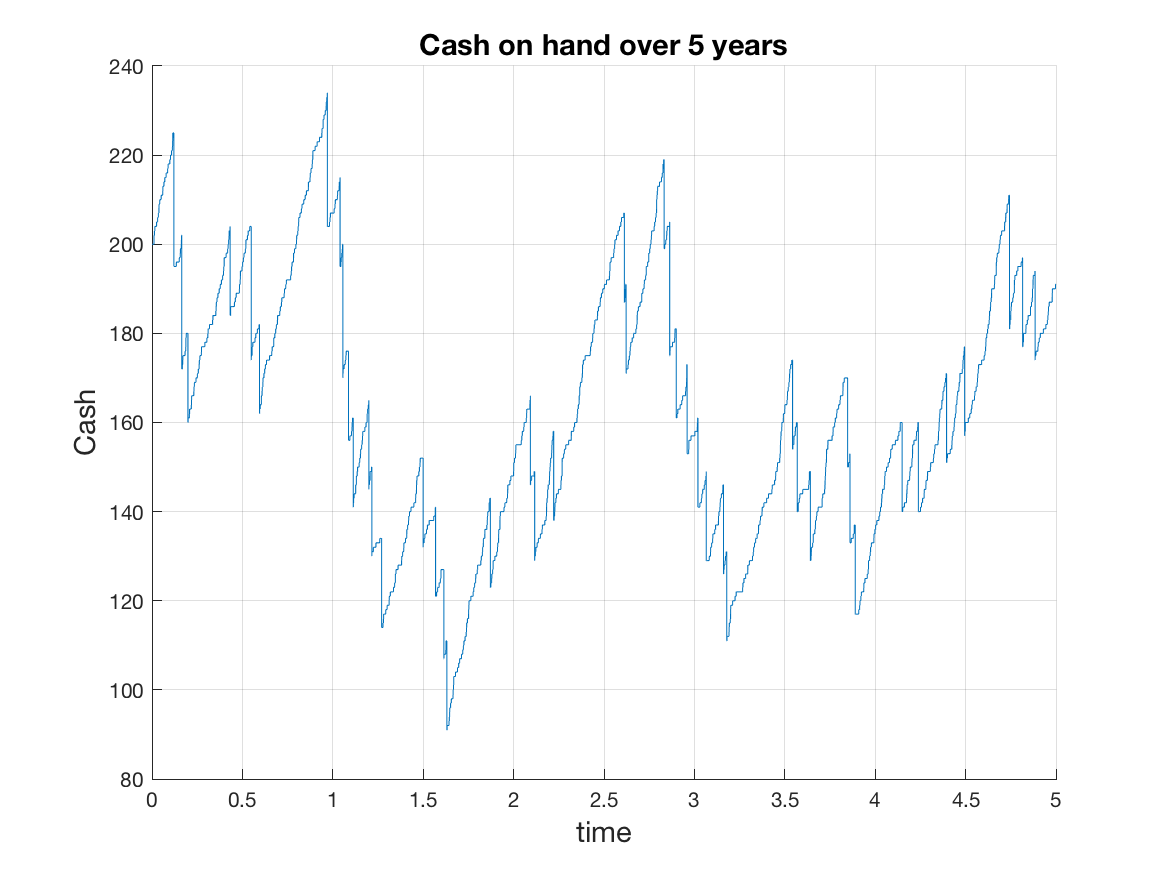
\includegraphics[width=0.7\linewidth]{figures/Cashflow}
	\caption{Cash On Hand @ time t}
	\label{fig:cashflow}
\end{figure}

\section{Kolmogorov's Forward Equation}
Given the lecture notes, 
\begin{center}
	\begin{tabular}{|| c | c | c | c ||} 
		\hline
		Range & State j @ t+1 & $v_x\cdot p_{xy}$ & $q_{xy}$\\ [0.5ex] 
		\hline\hline
		A & 1 & $\frac{\lambda}{\lambda} \cdot \lambda$ & $\lambda$ \\ 
		\hline
		B & x+1 & $\frac{\lambda}{\lambda + \alpha} \cdot (\lambda + \alpha)$ & $\lambda$\\
		\hline
		B & 0 & $\frac{\alpha}{\lambda + \alpha}\cdot (\lambda + \alpha)$ & $\alpha$ \\
		\hline
		C & x+1 & $\frac{\lambda}{\lambda + \alpha} \cdot (\lambda + \alpha)$ & $\lambda$\\
		\hline
		C & x-c & $\frac{\alpha}{\lambda + \alpha}\cdot (\lambda + \alpha)$ & $\alpha$\\
		\hline
		D & x-c & $\frac{\alpha}{\lambda + \beta + \alpha}\cdot (\lambda + \alpha + \beta)$& $\alpha$\\ 
		\hline
		D & x+1 & $\frac{\lambda}{\lambda + \beta + \alpha}\cdot (\lambda + \alpha + \beta)$& $\lambda$\\ 
		\hline
		D & x-d & $\frac{\beta}{\lambda + \beta + \alpha}\cdot (\lambda + \alpha + \beta)$& $\beta$\\ 
		\hline
		E & x-d & $\frac{\beta}{\beta + \alpha}\cdot (\beta + \alpha)$& $\beta$\\
		\hline
		E & x-c & $\frac{\alpha}{\beta + \alpha}\cdot (\beta + \alpha)$& $\alpha$\\[.5ex] 
		\hline
	\end{tabular}
\end{center}
Therefore, by plugging the various probabilities into the Kolmogorov's equations, I can generate the following:
\subsection{Range A, Y = 0}
$$\alpha\sum_{k=1}^{c} P_{xk}-\lambda P_{xy}$$
\subsection{Range B, 0 $<$ Y $<$ c}
$$\lambda P_{x,Y-1} + \alpha P_{x, Y+c} - (\lambda + \alpha)P_{xY}$$
\subsection{Range C, c $\leq$ Y $<$ X$_r$}
Given the dividend cannot surpass X$_r$,
$$\lambda P_{x,Y-1} + \alpha P_{x, Y+c} - (\lambda + \alpha)P_{xY}$$
Given the dividend can surpass X$_r$,
$$\lambda P_{x,Y-1} + \alpha P_{x, Y+c} + \beta P_{x, Y+d} - (\lambda + \alpha)P_{xY}$$
\subsection{Range D, X$_r$ $<$ Y $\leq$ Xmax}
The transition is close enough to Y that a claim or dividend can cause the transition:
$$\lambda P_{x,Y-1} + \alpha P_{x, Y+c} + \beta P_{x, Y+d} - (\lambda + \alpha + \beta)P_{xY}$$
When the transition cannot be caused by a claim or dividend:
$$\lambda P_{x,Y-1} - (\lambda + \alpha + \beta)P_{xY}$$
When a transition can only be caused a claim or premium:
$$\lambda P_{x,Y-1} + \alpha P_{x, Y+c} - (\lambda + \alpha + \beta)P_{xY}$$
When the transition can only be caused by a dividend or premium:
$$\lambda P_{x,Y-1} + \beta P_{x, Y+d} - (\lambda + \alpha + \beta)P_{xY}$$
\subsection{Range E, Y = Xmax}
$$\lambda P_{x,Y-1} - (\alpha + \beta)P_{xY}$$

\section{Kolmogorov's Backwards Equations}
\subsection{Range A, X = 0}
$$\lambda P_{X+1, y} - P_{X,y}$$
\subsection{Range B, 0 < X < c}
$$\lambda P_{X+1, y} + \alpha P_{0, y} - (\lambda + \alpha) P_{X,y}$$
\subsection{Range C, c $\leq$ X < X$_r$}
$$\lambda P_{X+1, y} + \alpha P_{x-c, y} - (\lambda + \alpha) P_{X,y}$$
\subsection{Range D, X$_r$ $\leq$ X $<$ Xmax}
$$\lambda P_{X+1, y} + \alpha P_{x-c, y} + \beta P_{x-d, y} - (\lambda + \alpha + \beta) P_{X,y}$$
\subsection{Range E, X = Xmax}
$$\alpha P_{x-c, y} + \beta P_{x-d, y} - (\alpha + \beta) P_{X,y}$$

\section{Solution of Kolmogorov’s equations}
\begin{lstlisting}
function [R]=Kolm(lambda,alpha,beta,c,d,Xr,Xmax)
	%UNTITLED2 Summary of this function goes here
	%   Detailed explanation goes here
	R=zeros(Xmax+1);
	R(1, 1) = -lambda;
	R(Xmax+1, Xmax)=lambda;
	R(Xmax+1, Xmax+1)=-(alpha+beta);
	
	for i=1:Xmax+1
		if i>=2 && i <=Xr-d
			R(i,i)=-(lambda+alpha);
			R(i, i-1) = lambda;
			R(i, i+c) = alpha;
		elseif i>=Xr-d+1 && i<=Xmax-d+1
			R(i, i-1) = lambda;
			R(i,i+c)=alpha;
			R(i,i+d)=beta;
			if i>= Xr+1
				R(i,i)=-(lambda+alpha+beta);
			else
				R(i,i)=-(lambda+alpha);
		end
			elseif i >= Xmax-d+2 && i<= Xmax-c+1
			R(i,i-1)=lambda;
			R(i,i+c)=alpha;
			R(i,i)=-(lambda+alpha+beta);
		elseif i>= Xmax-c+2 && i<=Xmax
			R(i,i-1)=lambda;
			R(i,i)=-(lambda+alpha+beta);
		end  
	end
end
\end{lstlisting}
The code above was used to generate the following: 
\begin{figure}[!ht]
	\centering
	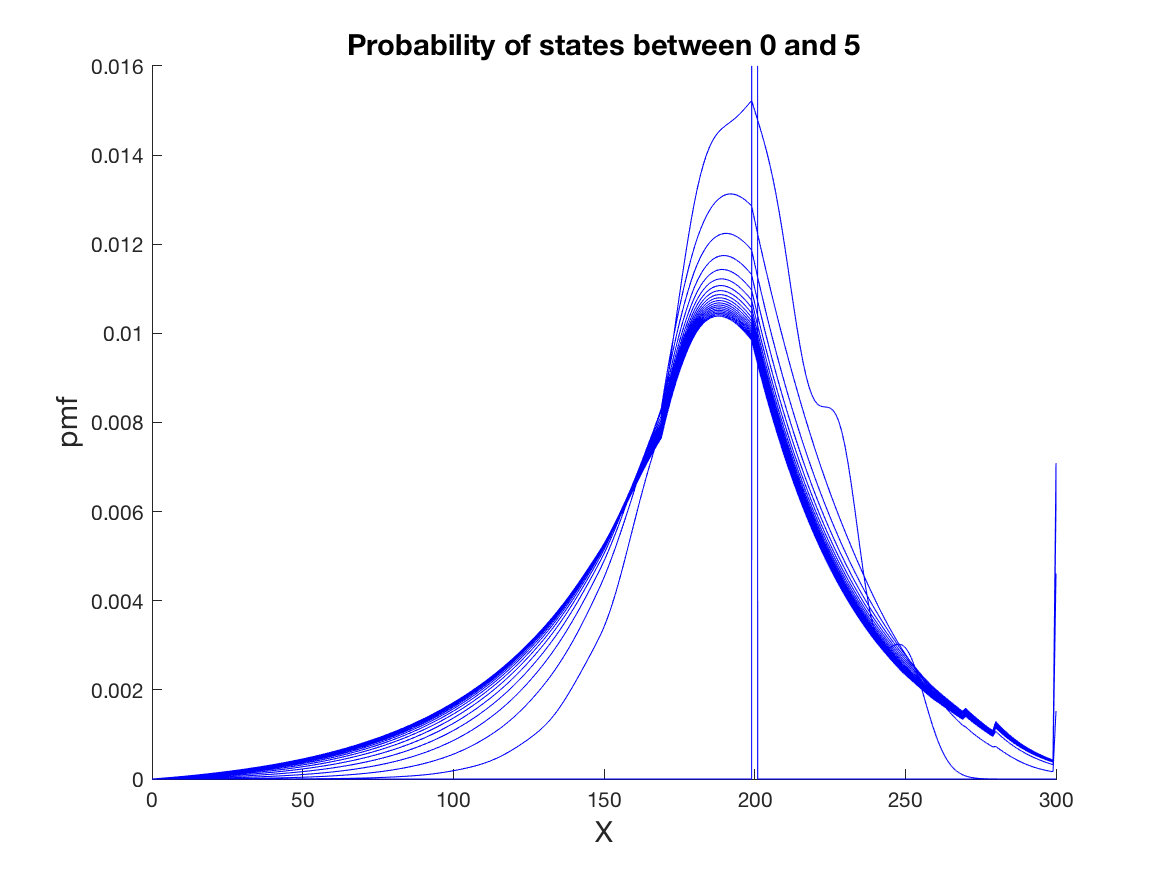
\includegraphics[width=0.7\linewidth]{figures/pmf}
	\caption{Probability Mass Function of Realizations}
	\label{fig:pmf}
\end{figure}
\pagebreak
\section{PMF of Dividends}
\begin{lstlisting}
s = 0;
for i=1:1000
[x,~] = cfSim(lambda,beta, alpha, X0, c, d, Xr, Xmax, Tmax);
a = x(2:end);
diff = a-x(1:end-1);
if ~isempty(find(diff == -d, 1))
s = s+1;
end
end
disp(s/100);

%%
pmf = zeros(100, 21);
for i=1:100
	[x,t] = cfSim(lambda,beta, alpha, X0, c, d, Xr, Xmax, Tmax);
	a = x(2:end);
	diff = a-x(1:end-1);
	
	T = .25:.25:5;
	edges = zeros(1, length(T));
	for tm = 1:length(T)
		[~,ind] = find(t<=T(tm), 1, 'last');
		edges(tm) = ind;
		end
		
		edges(edges > length(diff)) = length(diff);
		
		edges = [1,edges];
		p = zeros(1, 21);
		for e=2:21
		p(e-1) = length(find(diff(edges(e-1):edges(e)) == -d));
	end
	pmf(i, :) = p/sum(p);
end
pmf(any(isnan(pmf), 2),:)=[];
avg = mean(pmf);
stairs(0:20, avg);
grid on;
title('average pmf of paying a dividend at in quarter q (100 trials)');
xlabel('q');
ylabel('pmf');
saveas(gcf, 'pmfDividend.png');
\end{lstlisting}
The code above was used to generate the following: 
\begin{figure}[ht]
	\centering
	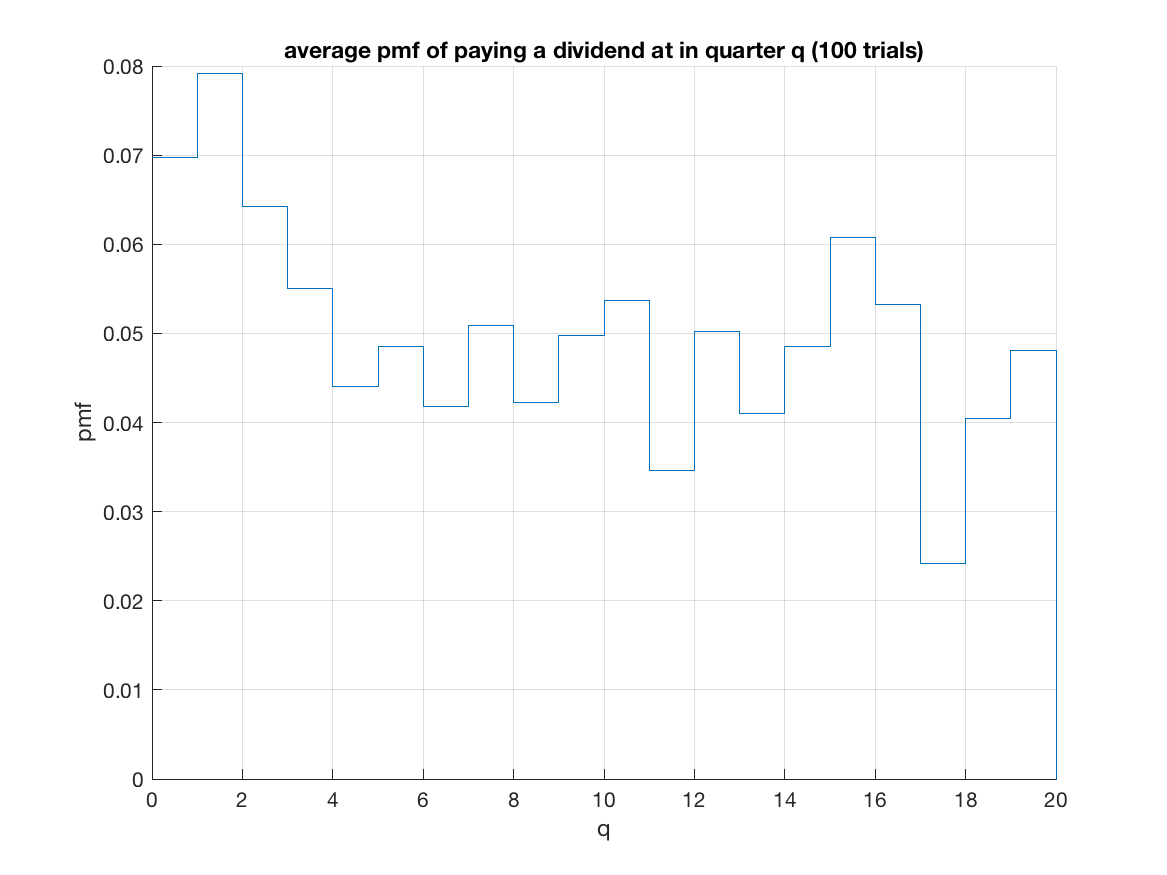
\includegraphics[width=0.7\linewidth]{figures/pmfDividend}
	\caption{Average pmf, 100 trials}
	\label{fig:pmfdividend}
\end{figure}
\pagebreak
\\
This indicates that over 20 quarters, the insurance company will almost always pay a dividend. However, the probability that the company will pay a dividend in quarter q varies from approx. 7.5\% to 3.75\% 


\end{document}
